\appendix

\section{Energy Evolution and Drift Plots}

\begin{figure}[ht]
	\centering
	\begin{minipage}[c]{\textwidth}
		\begin{center}
			\large Hagedorn Propagator \\[1mm]
			\normalsize Energy Evolution and Drift
			\vspace{4mm}
		\end{center}
	\end{minipage}
	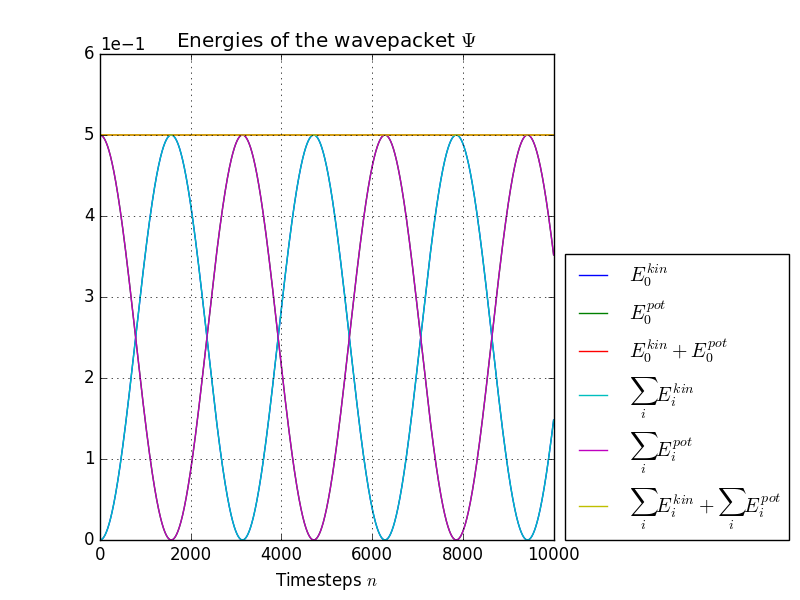
\includegraphics[width=.45\textwidth]{figures/harmonic_1D_Hagedorn_energies.png}
	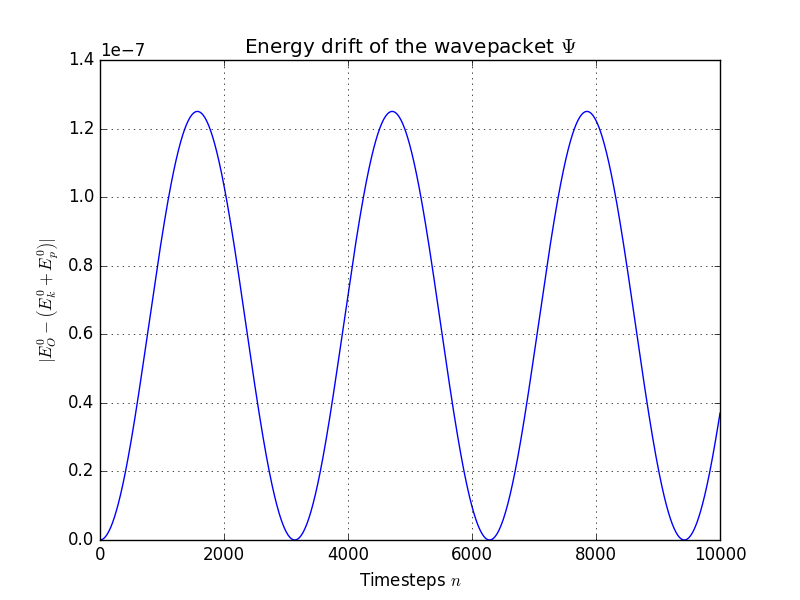
\includegraphics[width=.45\textwidth]{figures/harmonic_1D_Hagedorn_drift.png} \\
	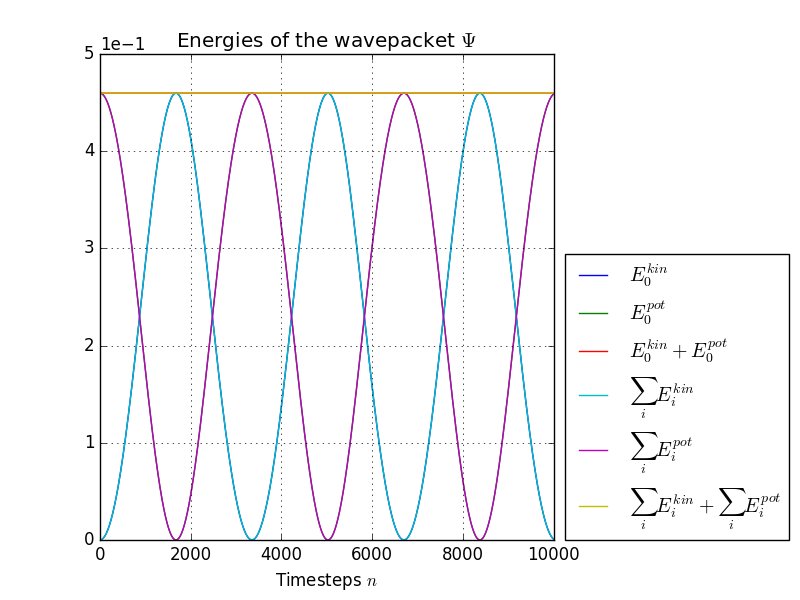
\includegraphics[width=.45\textwidth]{figures/torsional_1D_Hagedorn_energies.png}
	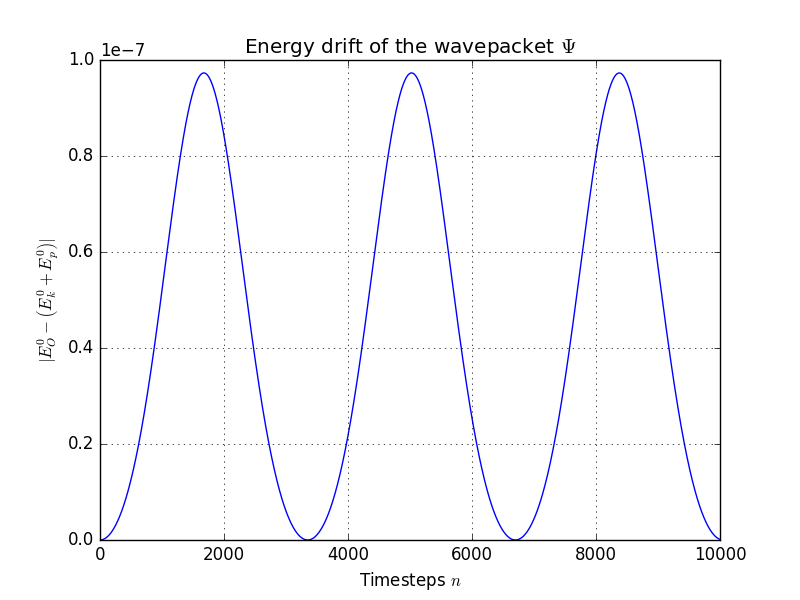
\includegraphics[width=.45\textwidth]{figures/torsional_1D_Hagedorn_drift.png} \\
	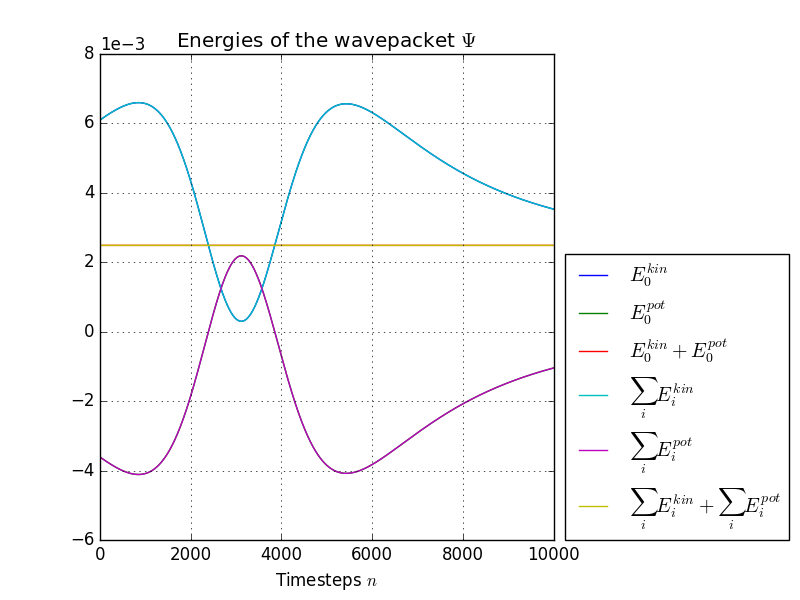
\includegraphics[width=.45\textwidth]{figures/morse_1D_Hagedorn_energies.png}
	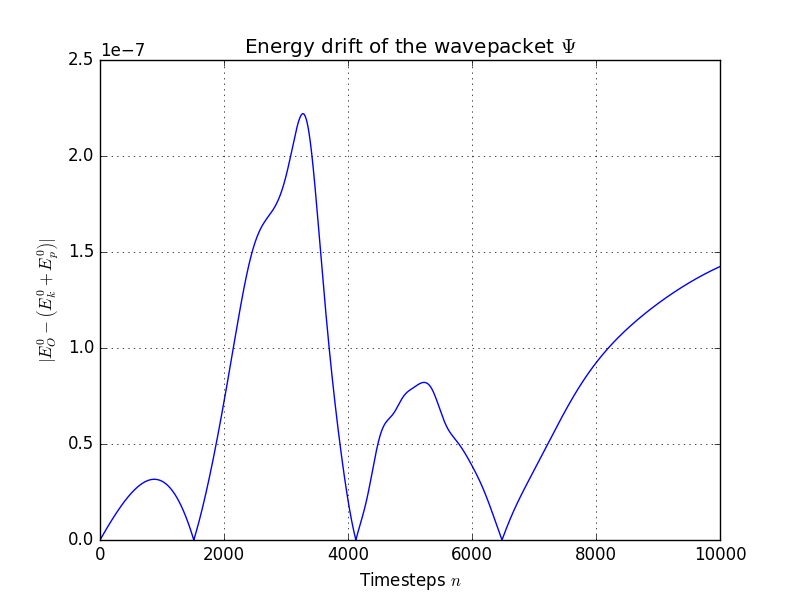
\includegraphics[width=.45\textwidth]{figures/morse_1D_Hagedorn_drift.png}
	\caption{Energy evolution and drift for a 1D wave packet propagated with the Hagedorn propagator in a harmonic potential (top), a torsional potential (middle) and a Morse potential (bottom).
	(Parameters: $N=1$, $D=1$ $|\K|=16$ $\eps=0.01$ (Morse $0.0484$), $T=10$ (Morse $T=50$), $\Dt=0.001$ (Morse $\Dt=0.005$), Hagedorn propagator)}
	\label{fig:energy_Hagedorn}
\end{figure}
%
\begin{figure}[ht]
	\centering
	\begin{minipage}[c]{\textwidth}
		\begin{center}
			\large MG4 Propagator \\[1mm]
			\normalsize Energy Evolution and Drift
			\vspace{4mm}
		\end{center}
	\end{minipage}
	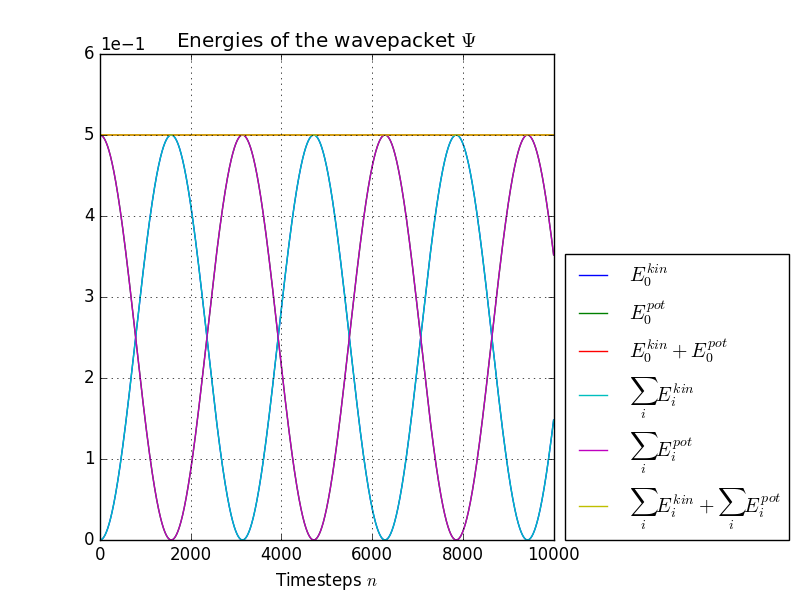
\includegraphics[width=.45\textwidth]{figures/harmonic_1D_MG4_energies.png}
	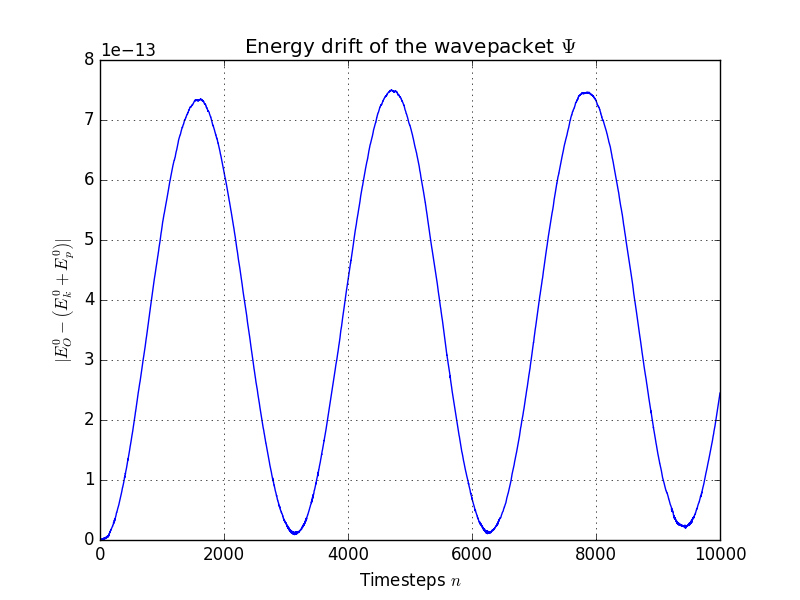
\includegraphics[width=.45\textwidth]{figures/harmonic_1D_MG4_drift.png} \\
	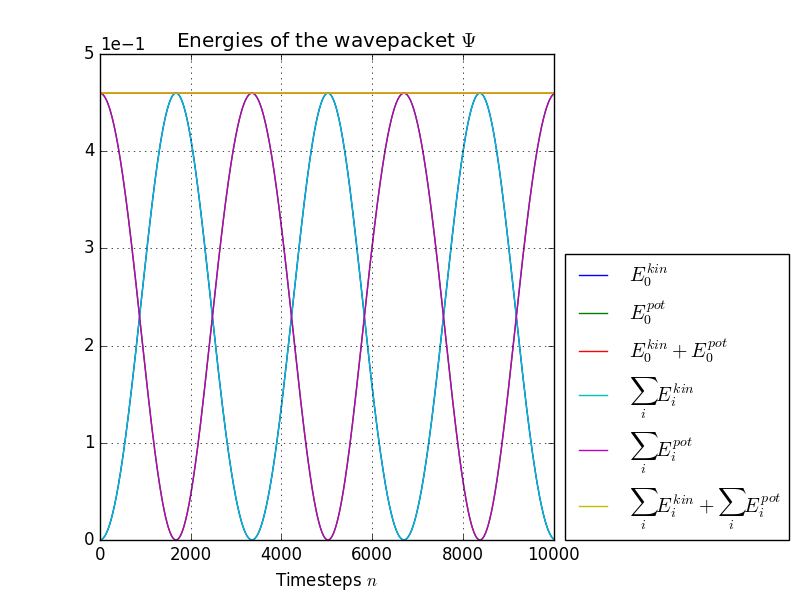
\includegraphics[width=.45\textwidth]{figures/torsional_1D_MG4_energies.png}
	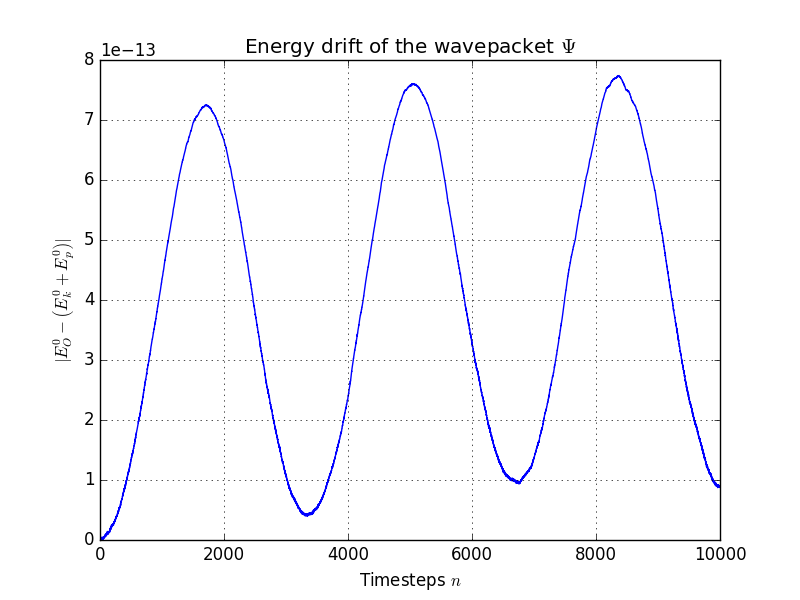
\includegraphics[width=.45\textwidth]{figures/torsional_1D_MG4_drift.png} \\
	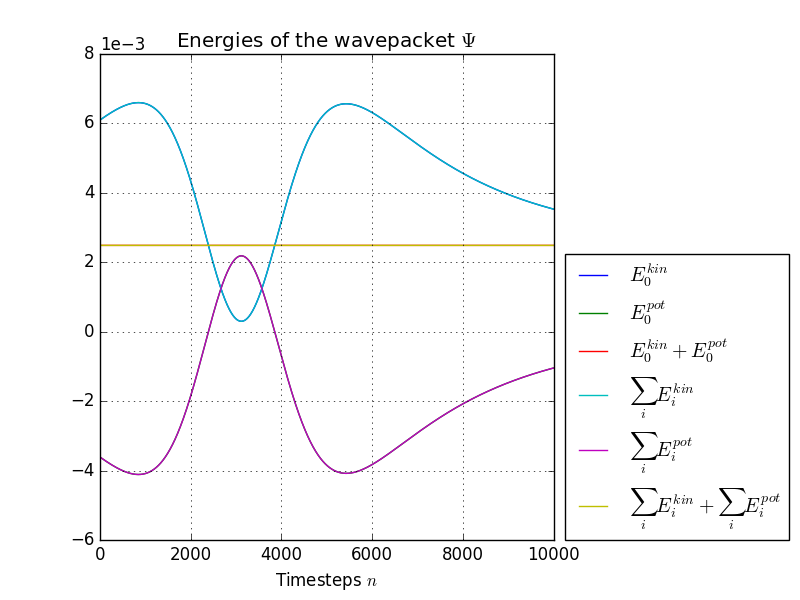
\includegraphics[width=.45\textwidth]{figures/morse_1D_MG4_energies.png}
	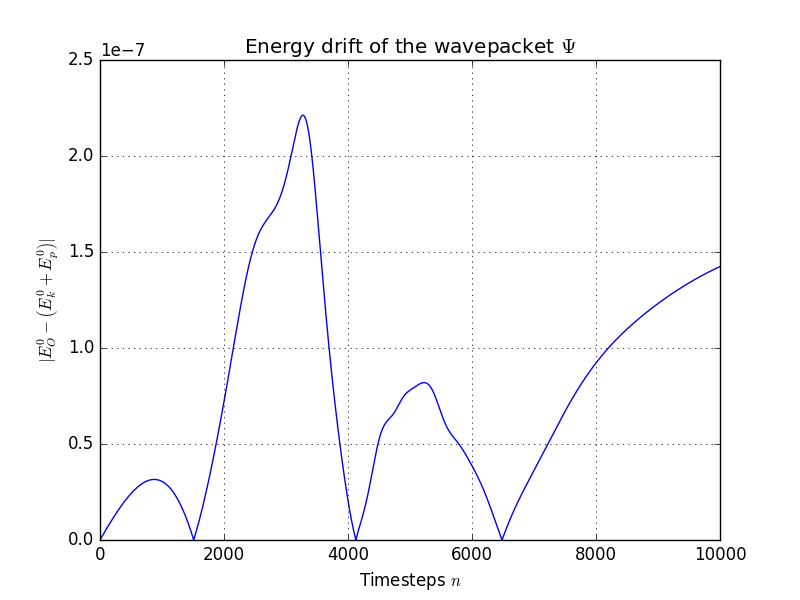
\includegraphics[width=.45\textwidth]{figures/morse_1D_MG4_drift.png}
	\caption{Energy evolution and drift for a 1D wave packet propagated with the MG4 propagator in a harmonic potential (top), a torsional potential (middle) and a Morse potential (bottom).
	(Parameters: $N=1$, $D=1$ $|\K|=16$ $\eps=0.01$ (Morse $0.0484$), $T=10$ (Morse $T=50$), $\Dt=0.001$ (Morse $\Dt=0.005$), MG4 propagator with \emph{Y4} splitting for \proc{IntSplit})}
	\label{fig:energy_MG4}
\end{figure}
%
\begin{figure}[ht]
	\centering
	\begin{minipage}[c]{\textwidth}
		\begin{center}
			\large McL42 Propagator \\[1mm]
			\normalsize Energy Evolution and Drift
			\vspace{4mm}
		\end{center}
	\end{minipage}
	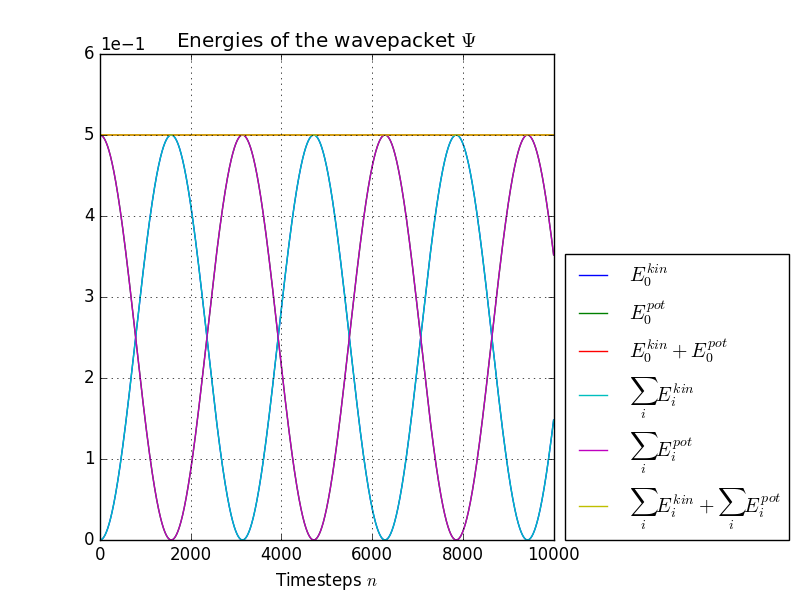
\includegraphics[width=.45\textwidth]{figures/harmonic_1D_McL42_energies.png}
	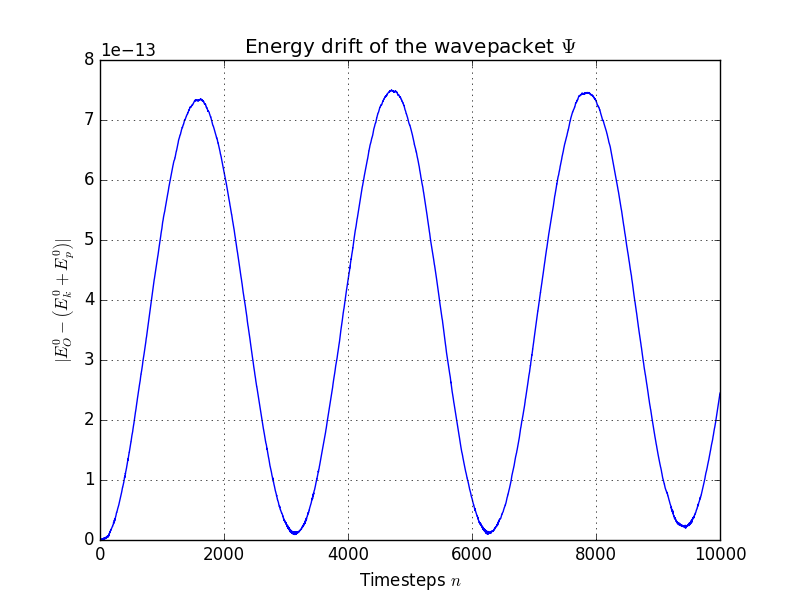
\includegraphics[width=.45\textwidth]{figures/harmonic_1D_McL42_drift.png} \\
	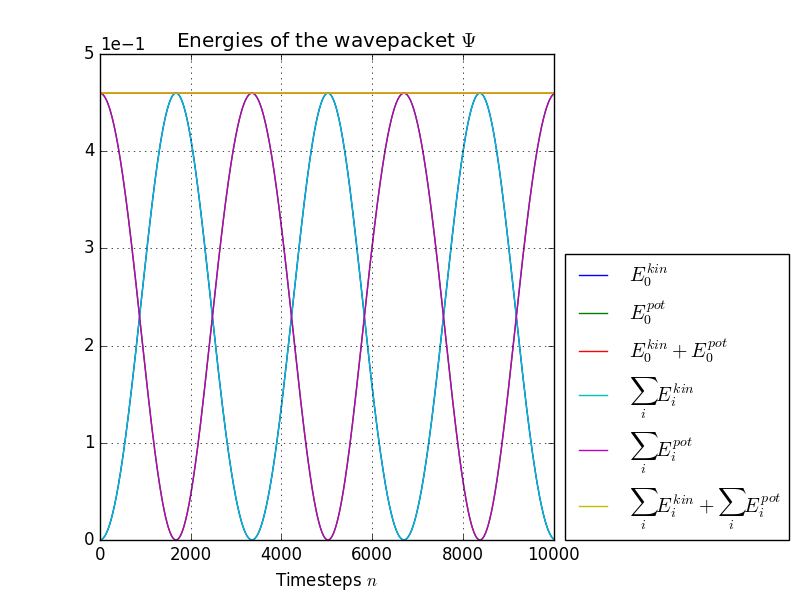
\includegraphics[width=.45\textwidth]{figures/torsional_1D_McL42_energies.png}
	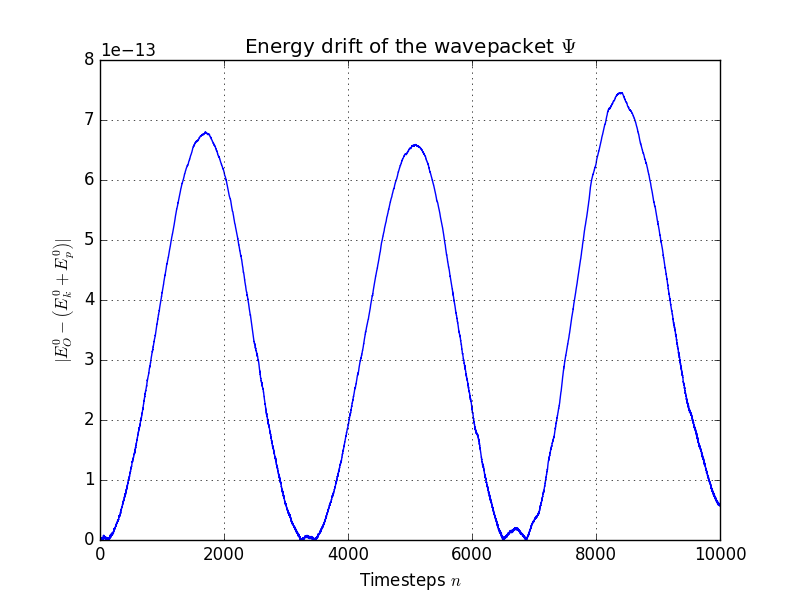
\includegraphics[width=.45\textwidth]{figures/torsional_1D_McL42_drift.png} \\
	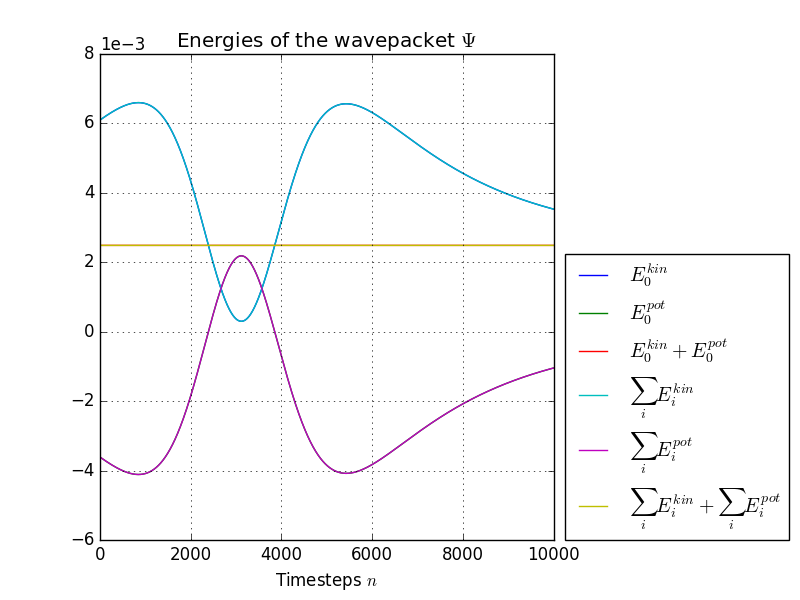
\includegraphics[width=.45\textwidth]{figures/morse_1D_McL42_energies.png}
	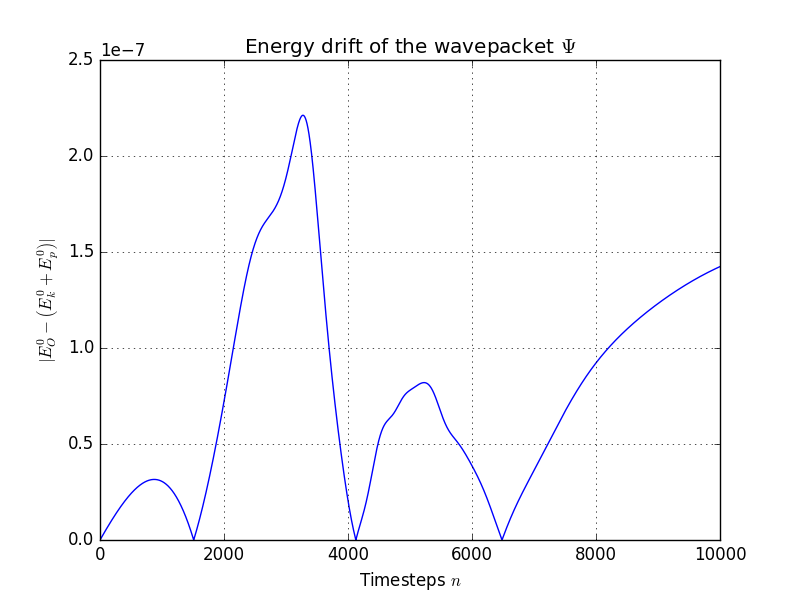
\includegraphics[width=.45\textwidth]{figures/morse_1D_McL42_drift.png}
	\caption{Energy evolution and drift for a 1D wave packet propagated with the McL42 propagator in a harmonic potential (top), a torsional potential (middle) and a Morse potential (bottom).
	(Parameters: $N=1$, $D=1$ $|\K|=16$ $\eps=0.01$ (Morse $0.0484$), $T=10$ (Morse $T=50$), $\Dt=0.001$ (Morse $\Dt=0.005$), McL42 propagator with \emph{Y4} splitting for \proc{IntSplit})}
	\label{fig:energy_McL42}
\end{figure}
%
\begin{figure}[ht]
	\centering
	\begin{minipage}[c]{\textwidth}
		\begin{center}
			\large McL84 Propagator \\[1mm]
			\normalsize Energy Evolution and Drift
			\vspace{4mm}
		\end{center}
	\end{minipage}
	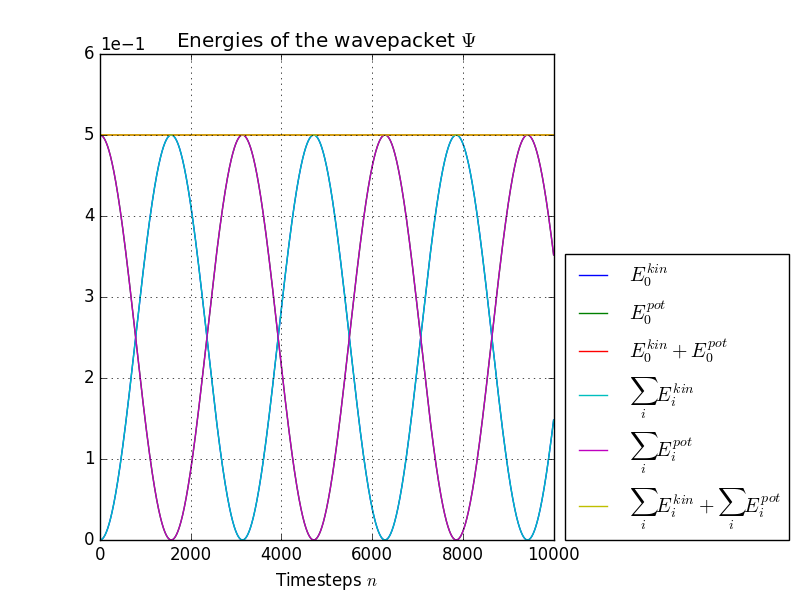
\includegraphics[width=.45\textwidth]{figures/harmonic_1D_McL84_energies.png}
	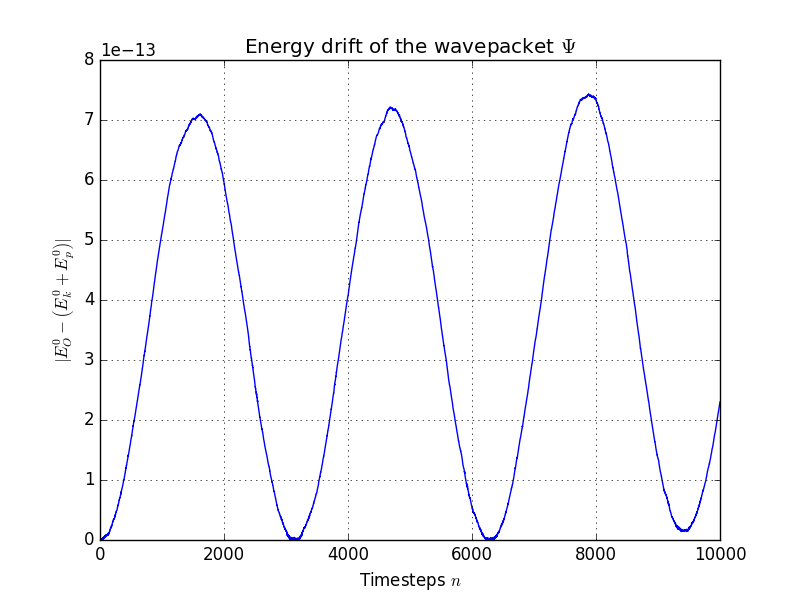
\includegraphics[width=.45\textwidth]{figures/harmonic_1D_McL84_drift.png} \\
	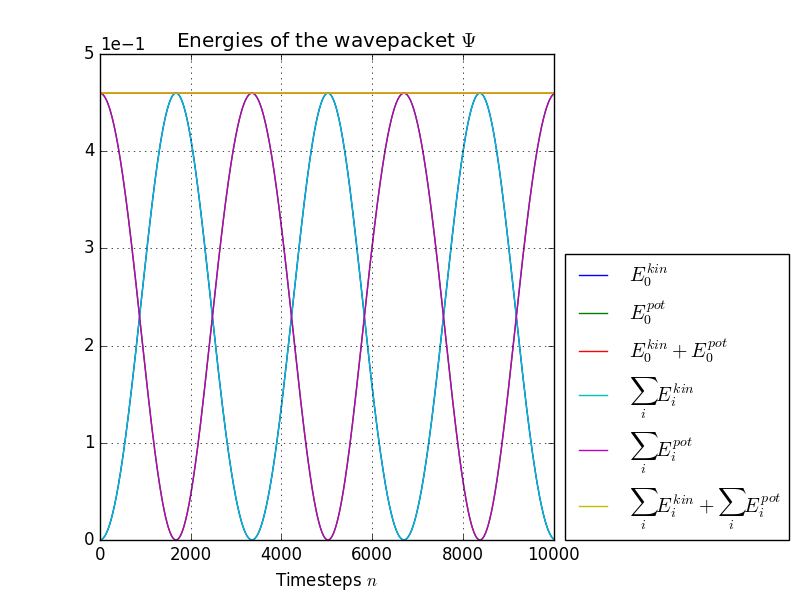
\includegraphics[width=.45\textwidth]{figures/torsional_1D_McL84_energies.png}
	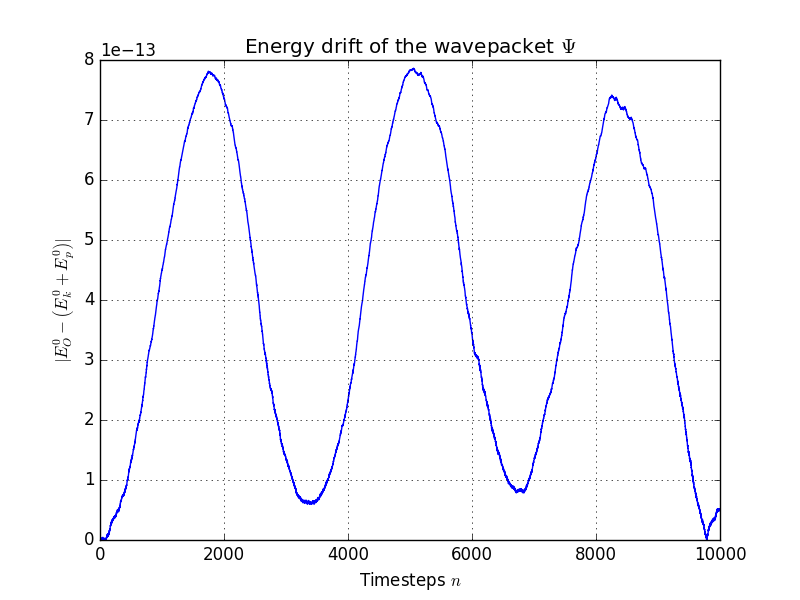
\includegraphics[width=.45\textwidth]{figures/torsional_1D_McL84_drift.png} \\
	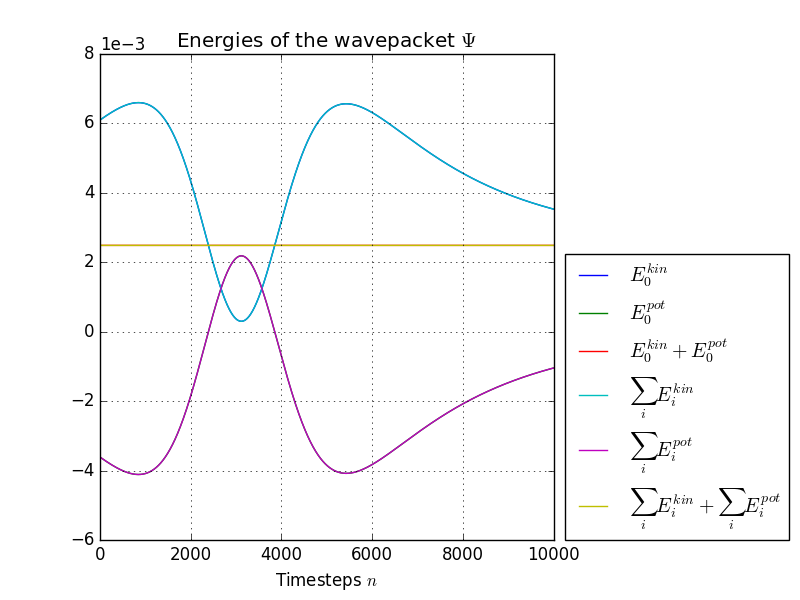
\includegraphics[width=.45\textwidth]{figures/morse_1D_McL84_energies.png}
	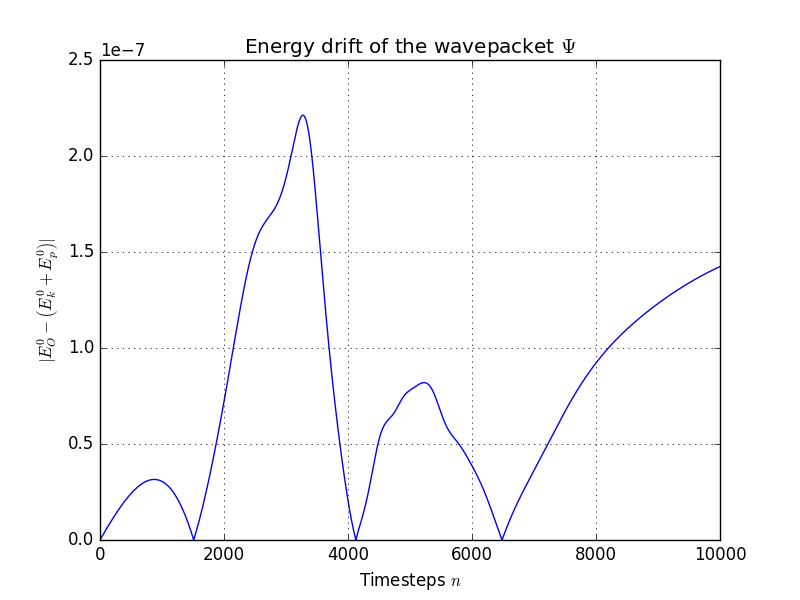
\includegraphics[width=.45\textwidth]{figures/morse_1D_McL84_drift.png}
	\caption{Energy evolution and drift for a 1D wave packet propagated with the McL84 propagator in a harmonic potential (top), a torsional potential (middle) and a Morse potential (bottom).
	(Parameters: $N=1$, $D=1$ $|\K|=16$ $\eps=0.01$ (Morse $0.0484$), $T=10$ (Morse $T=50$), $\Dt=0.001$ (Morse $\Dt=0.005$), McL84 propagator with \emph{Y4} splitting for \proc{IntSplit})}
	\label{fig:energy_McL84}
\end{figure}
%
\begin{figure}[ht]
	\centering
	\begin{minipage}[c]{\textwidth}
		\begin{center}
			\large Pre764 Propagator \\[1mm]
			\normalsize Energy Evolution and Drift
			\vspace{4mm}
		\end{center}
	\end{minipage}
	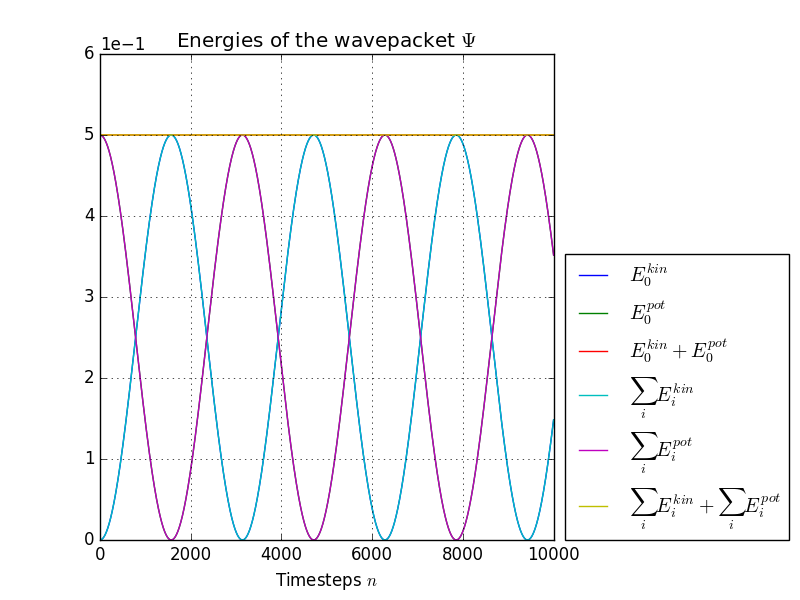
\includegraphics[width=.45\textwidth]{figures/harmonic_1D_Pre764_energies.png}
	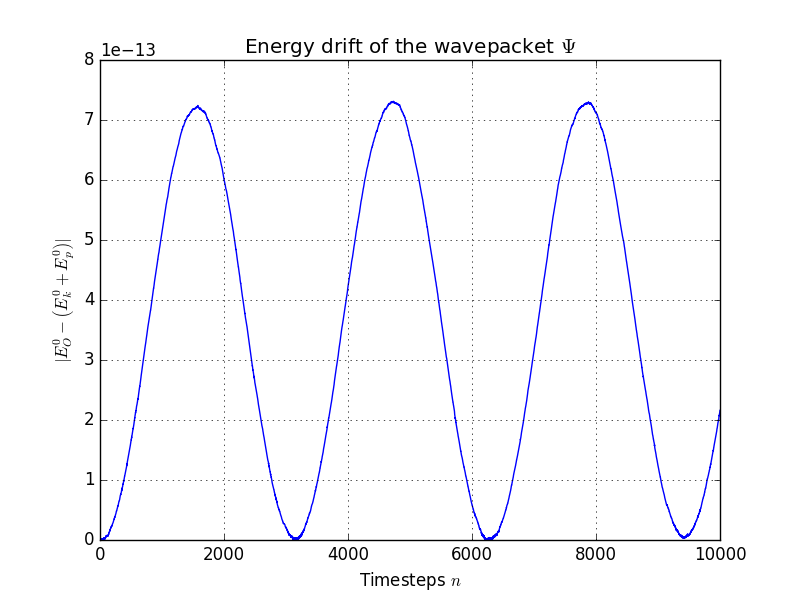
\includegraphics[width=.45\textwidth]{figures/harmonic_1D_Pre764_drift.png} \\
	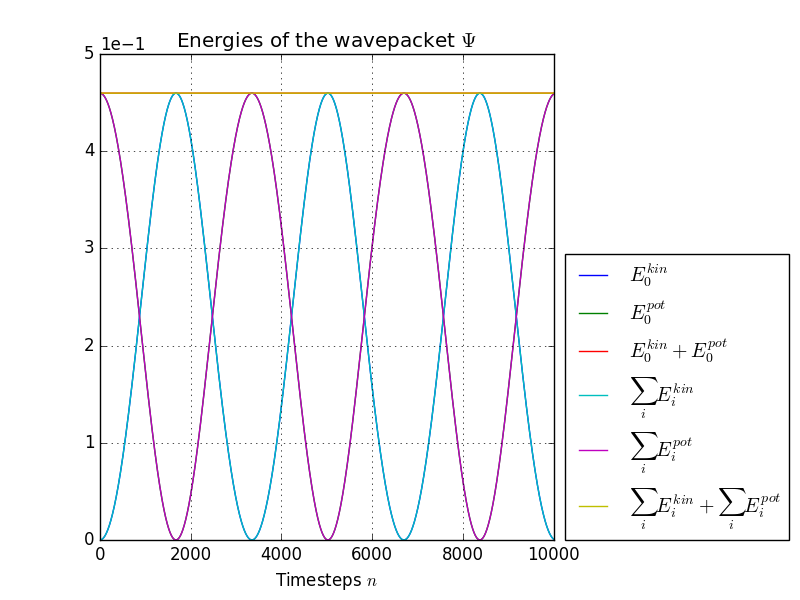
\includegraphics[width=.45\textwidth]{figures/torsional_1D_Pre764_energies.png}
	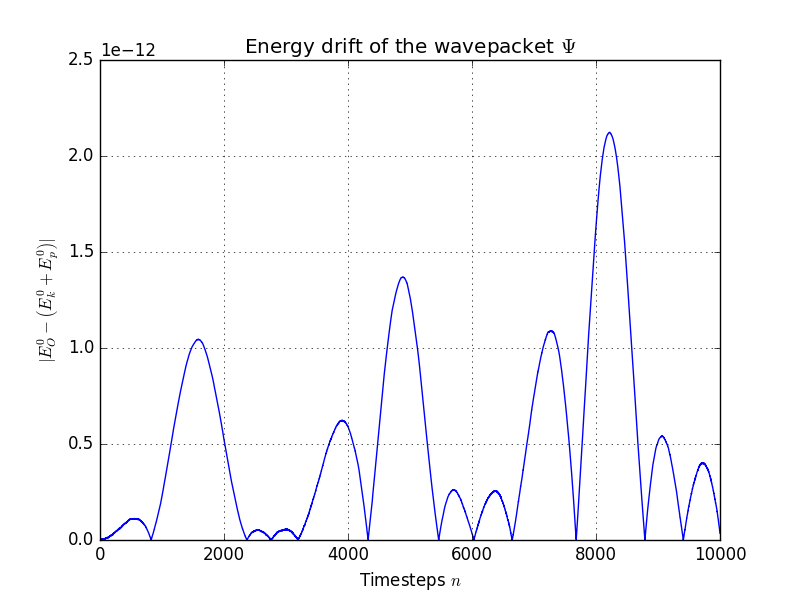
\includegraphics[width=.45\textwidth]{figures/torsional_1D_Pre764_drift.png} \\
	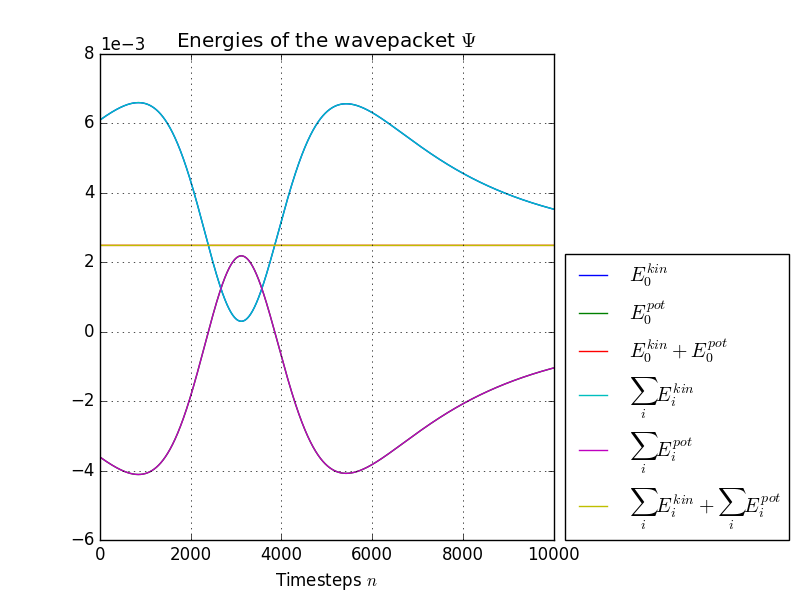
\includegraphics[width=.45\textwidth]{figures/morse_1D_Pre764_energies.png}
	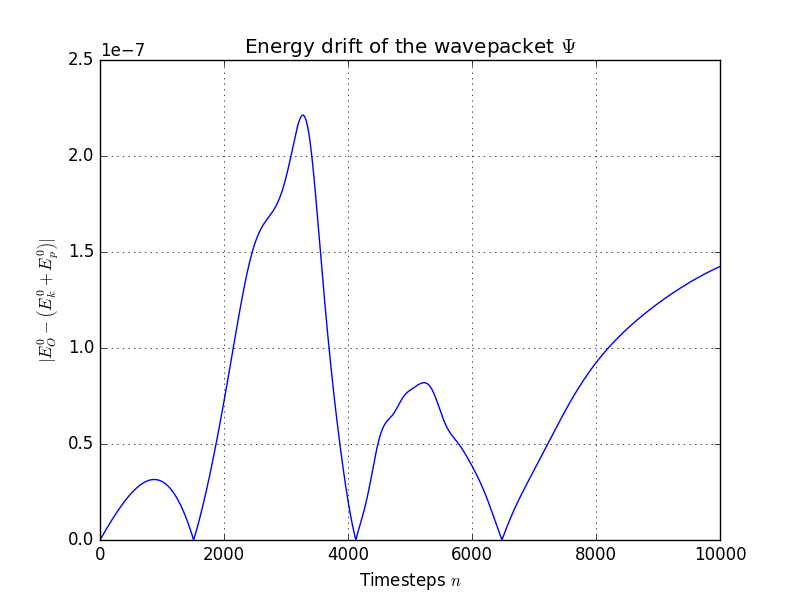
\includegraphics[width=.45\textwidth]{figures/morse_1D_Pre764_drift.png}
	\caption{Energy evolution and drift for a 1D wave packet propagated with the Pre764 propagator in a harmonic potential (top), a torsional potential (middle) and a Morse potential (bottom).
	(Parameters: $N=1$, $D=1$ $|\K|=16$ $\eps=0.01$ (Morse $0.0484$), $T=10$ (Morse $T=50$), $\Dt=0.001$ (Morse $\Dt=0.005$), Pre764 propagator with \emph{Y4} splitting for \proc{IntSplit})}
	\label{fig:energy_Pre764}
\end{figure}
